%%% Fiktivní kapitola s ukázkami sazby

\chapter{Tipy k psaní, ukázky sazby}

\section{Pomlčky, no-breaky, jednotky, uvozovky}

Čísla v~českém textu obvykle sázíme v~matematickém režimu s~desetinnou čárkou:
%%% Bez \usepackage{icomma}:
% $\pi \doteq 3{,}141\,592\,653\,589$.
%%% S \usepackage{icomma}:
$\pi \doteq 3,141\,592\,653\,589$.
V~matematických textech se považuje za přípustné používat desetinnou tečku
(pro lepší odlišení od čárky v~roli oddělovače). Numerické výsledky se uvádějí
s~přiměřeným počtem desetinných míst.

Mezi číslo a jednotku patří úzká mezera: šířka stránky A4 činí $210\,\rm mm$, což si
pamatuje pouze $5\,\%$ autorů. Pokud ale údaj slouží jako přívlastek, mezeru vynecháváme:
$25\rm mm$ okraj, $95\%$ interval spolehlivosti.

Rozlišujeme různé druhy pomlček:
červeno-černý (krátká pomlčka),
strana 16--22 (střední),
$45-44$ (matematické minus),
a~toto je --- jak se asi dalo čekat --- vložená věta ohraničená dlouhými pomlčkami.

V~českém textu se používají \uv{české} uvozovky, nikoliv ``anglické''.

% V tomto odstavci se vlnka zviditelňuje
{
\def~{{\tt\char126}}
Na některých místech je potřeba zabránit lámání řádku (v~\TeX{}u značíme vlnovkou):
u~předložek (neslabičnych, nebo obecně jednopísmenných), vrchol~$v$, před $k$~kroky,
a~proto, \dots{} obecně kdekoliv, kde by při rozlomení čtenář \uv{ško\-brt\-nul}.
}

\section{Matematické vzorce a výrazy}

Proměnné sázíme kurzívou (to \TeX{} v~matematickém módu dělá sám, ale
nezapomínejte na to v~okolním textu a také si matematický mód zapněte).
Názvy funkcí sázíme vzpřímeně. Tedy například:
$\var(X) = \E X^2 - \bigl(\E X \bigr)^2$.

Zlomky uvnitř odstavce (třeba $\frac{5}{7}$ nebo $\frac{x+y}{2}$) mohou
být příliš stísněné, takže je lepší sázet jednoduché zlomky s~lomítkem:
$5/7$, $(x+y)/2$.

Nechť
\[   % LaTeXová náhrada klasického TeXového $$
\mathbb{X} = \begin{pmatrix}
      \T{\bm x_1} \\
      \vdots \\
      \T{\bm x_n}
      \end{pmatrix}.
\]
Povšimněme si tečky za~maticí. Byť je matematický text vysázen
ve~specifickém prostředí, stále je gramaticky součástí věty a~tudíž je
zapotřebí neopomenout patřičná interpunkční znaménka. Výrazy, na které
chceme později odkazovat, je vhodné očíslovat:
\begin{equation}\label{eq01:Xmat}
\mathbb{X} = \begin{pmatrix}
      \T{\bm x_1} \\
      \vdots \\
      \T{\bm x_n}
      \end{pmatrix}.
\end{equation}
Výraz \eqref{eq01:Xmat} definuje matici $\mathbb{X}$. Pro lepší čitelnost
a~přehlednost textu je vhodné číslovat pouze ty výrazy, na které se
autor někde v~další části textu odkazuje. To jest, nečíslujte
automaticky všechny výrazy vysázené některým z~matematických
prostředí.

Zarovnání vzorců do několika sloupečků:
\begin{alignat*}{3}
S(t) &= \pr(T > t),    &\qquad t&>0       &\qquad&\text{ (zprava spojitá),}\\
F(t) &= \pr(T \leq t), &\qquad t&>0       &\qquad&\text{ (zprava spojitá).}
\end{alignat*}

Dva vzorce se spojovníkem:
\begin{equation}\label{eq01:FS}
\left.
\begin{aligned}
S(t) &= \pr(T > t) \\[1ex]
F(t) &= \pr(T \leq t)
\end{aligned}
\;	% zde pomůže ručně vynechat trochu místa
\right\}
\quad t>0 \qquad \text{(zprava spojité).}
\end{equation}

Dva centrované nečíslované vzorce:
\begin{gather*}
\bm Y = \mathbb{X}\bm\beta + \bm\varepsilon, \\[1ex]
\mathbb{X} = \begin{pmatrix} 1 & \T{\bm x_1} \\ \vdots & \vdots \\ 1 &
  \T{\bm x_n} \end{pmatrix}.
\end{gather*}
Dva centrované číslované vzorce:
\begin{gather}
\bm Y = \mathbb{X}\bm\beta + \bm\varepsilon, \label{eq02:Y}\\[1ex]
\mathbb{X} = \begin{pmatrix} 1 & \T{\bm x_1} \label{eq03:X}\\ \vdots & \vdots \\ 1 &
  \T{\bm x_n} \end{pmatrix}.
\end{gather}

Definice rozdělená na dva případy:
\[
P_{r-j}=
\begin{cases}
0, & \text{je-li $r-j$ liché},\\
r!\,(-1)^{(r-j)/2}, & \text{je-li $r-j$ sudé}.
\end{cases}
\]
Všimněte si použití interpunkce v této konstrukci. Čárky a tečky se
dávají na místa, kam podle jazykových pravidel patří.

\begin{align}
x& = y_1-y_2+y_3-y_5+y_8-\dots = && \text{z \eqref{eq02:Y}} \nonumber\\
& = y'\circ y^* = && \text{podle \eqref{eq03:X}} \nonumber\\
& = y(0) y' && \text {z Axiomu 1.}
\end{align}


Dva zarovnané vzorce nečíslované:
\begin{align*}
L(\bm\theta) &= \prod_{i=1}^n f_i(y_i;\,\bm\theta), \\
\ell(\bm\theta) &= \log\bigl\{L(\bm\theta)\bigr\} =
\sum_{i=1}^n \log\bigl\{f_i(y_i;\,\bm\theta)\bigr\}.
\end{align*}
Dva zarovnané vzorce, první číslovaný:
\begin{align}
L(\bm\theta) &= \prod_{i=1}^n f_i(y_i;\,\bm\theta), \label{eq01:L} \\
\ell(\bm\theta) &= \log\bigl\{L(\bm\theta)\bigr\} =
\sum_{i=1}^n \log\bigl\{f_i(y_i;\,\bm\theta)\bigr\}. \nonumber
\end{align}

Vzorec na dva řádky, první řádek zarovnaný vlevo, druhý vpravo, nečíslovaný:
\begin{multline*}
\ell(\mu,\,\sigma^2) = \log\bigl\{L(\mu,\,\sigma^2)\bigr\} =
\sum_{i=1}^n \log\bigl\{f_i(y_i;\,\mu,\,\sigma^2)\bigr\}= \\
  = -\,\frac{n}{2}\,\log(2\pi\sigma^2) \,-\,
\frac{1}{2\sigma^2}\sum_{i=1}^n\,(y_i - \mu)^2.
\end{multline*}

Vzorec na dva řádky, zarovnaný na $=$, číslovaný uprostřed:
\begin{equation}\label{eq01:ell}
\begin{split}
\ell(\mu,\,\sigma^2) &= \log\bigl\{L(\mu,\,\sigma^2)\bigr\} =
\sum_{i=1}^n \log\bigl\{f(y_i;\,\mu,\,\sigma^2)\bigr\}= \\
& = -\,\frac{n}{2}\,\log(2\pi\sigma^2) \,-\,
\frac{1}{2\sigma^2}\sum_{i=1}^n\,(y_i - \mu)^2.
\end{split}
\end{equation}

\section{Definice, věty, důkazy, \dots}

Konstrukce typu definice, věta, důkaz, příklad, \dots je vhodné
odlišit od okolního textu a~případně též číslovat s~možností použití
křížových odkazů. Pro každý typ těchto konstrukcí je vhodné mít
v~souboru s~makry (\texttt{makra.tex}) nadefinované jedno prostředí,
které zajistí jak vizuální odlišení od okolního textu, tak
automatické číslování s~možností křížově odkazovat.

\begin{definice}\label{def01:1}
  Nechť náhodné veličiny $X_1,\dots,X_n$ jsou definovány na témž
  prav\-dě\-po\-dob\-nost\-ním prostoru $(\Omega,\,\mathcal{A},\,\pr)$. Pak
  vektor $\bm X = \T{(X_1,\dots,X_n)}$ nazveme \emph{náhodným
    vektorem}.
\end{definice}

\begin{definice}[náhodný vektor]\label{def01:2}
  Nechť náhodné veličiny $X_1,\dots,X_n$ jsou definovány na témž
  pravděpodobnostním prostoru $(\Omega,\,\mathcal{A},\,\pr)$. Pak
  vektor $\bm X = \T{(X_1,\dots,X_n)}$ nazveme \emph{náhodným
    vektorem}.
\end{definice}
Definice~\ref{def01:1} ukazuje použití prostředí pro sazbu definice
bez titulku, definice~\ref{def01:2} ukazuje použití prostředí pro
sazbu definice s~titulkem.

\begin{veta}\label{veta01:1}
  Náhodný vektor $\bm X$ je měřitelné zobrazení prostoru
  $(\Omega,\,\mathcal{A},\,\pr)$ do $(\R_n,\,\mathcal{B}_n)$.
\end{veta}

\begin{lemma}[\citealp{Andel07}, str. 29]\label{veta01:2}
  Náhodný vektor $\bm X$ je měřitelné zobrazení prostoru
  $(\Omega,\,\mathcal{A},\,\pr)$ do $(\R_n,\,\mathcal{B}_n)$.
\end{lemma}
\begin{dukaz}
  Jednotlivé kroky důkazu jsou podrobně popsány v~práci \citet[str.
  29]{Andel07}.
\end{dukaz}
Věta~\ref{veta01:1} ukazuje použití prostředí pro sazbu matematické
věty bez titulku, lemma~\ref{veta01:2} ukazuje použití prostředí pro
sazbu matematické věty s~titulkem. Lemmata byla zavedena v~hlavním
souboru tak, že sdílejí číslování s~větami.
 
\section{Matematické vzorce a výrazy}

Proměnné sázíme kurzívou (to \TeX{} v~matematickém módu dělá sám, ale
nezapomínejte na to v~okolním textu a také si matematický mód zapněte).
Názvy funkcí sázíme vzpřímeně. Tedy například:
$\var(X) = \E X^2 - \bigl(\E X \bigr)^2$.

Zlomky uvnitř odstavce (třeba $\frac{5}{7}$ nebo $\frac{x+y}{2}$) mohou
být příliš stísněné, takže je lepší sázet jednoduché zlomky s~lomítkem:
$5/7$, $(x+y)/2$.

Nechť
\[   % LaTeXová náhrada klasického TeXového $$
\mathbb{X} = \begin{pmatrix}
      \T{\bm x_1} \\
      \vdots \\
      \T{\bm x_n}
      \end{pmatrix}.
\]
Povšimněme si tečky za~maticí. Byť je matematický text vysázen
ve~specifickém prostředí, stále je gramaticky součástí věty a~tudíž je
zapotřebí neopomenout patřičná interpunkční znaménka. Výrazy, na které
chceme později odkazovat, je vhodné očíslovat:
\begin{equation}\label{eq01:Xmat}
\mathbb{X} = \begin{pmatrix}
      \T{\bm x_1} \\
      \vdots \\
      \T{\bm x_n}
      \end{pmatrix}.
\end{equation}
Výraz \eqref{eq01:Xmat} definuje matici $\mathbb{X}$. Pro lepší čitelnost
a~přehlednost textu je vhodné číslovat pouze ty výrazy, na které se
autor někde v~další části textu odkazuje. To jest, nečíslujte
automaticky všechny výrazy vysázené některým z~matematických
prostředí.

Zarovnání vzorců do několika sloupečků:
\begin{alignat*}{3}
S(t) &= \pr(T > t),    &\qquad t&>0       &\qquad&\text{ (zprava spojitá),}\\
F(t) &= \pr(T \leq t), &\qquad t&>0       &\qquad&\text{ (zprava spojitá).}
\end{alignat*}

Dva vzorce se spojovníkem:
\begin{equation}\label{eq01:FS}
\left.
\begin{aligned}
S(t) &= \pr(T > t) \\[1ex]
F(t) &= \pr(T \leq t)
\end{aligned}
\;	% zde pomůže ručně vynechat trochu místa
\right\}
\quad t>0 \qquad \text{(zprava spojité).}
\end{equation}

Dva centrované nečíslované vzorce:
\begin{gather*}
\bm Y = \mathbb{X}\bm\beta + \bm\varepsilon, \\[1ex]
\mathbb{X} = \begin{pmatrix} 1 & \T{\bm x_1} \\ \vdots & \vdots \\ 1 &
  \T{\bm x_n} \end{pmatrix}.
\end{gather*}
Dva centrované číslované vzorce:
\begin{gather}
\bm Y = \mathbb{X}\bm\beta + \bm\varepsilon, \label{eq02:Y}\\[1ex]
\mathbb{X} = \begin{pmatrix} 1 & \T{\bm x_1} \label{eq03:X}\\ \vdots & \vdots \\ 1 &
  \T{\bm x_n} \end{pmatrix}.
\end{gather}

Definice rozdělená na dva případy:
\[
P_{r-j}=
\begin{cases}
0, & \text{je-li $r-j$ liché},\\
r!\,(-1)^{(r-j)/2}, & \text{je-li $r-j$ sudé}.
\end{cases}
\]
Všimněte si použití interpunkce v této konstrukci. Čárky a tečky se
dávají na místa, kam podle jazykových pravidel patří.

\begin{align}
x& = y_1-y_2+y_3-y_5+y_8-\dots = && \text{z \eqref{eq02:Y}} \nonumber\\
& = y'\circ y^* = && \text{podle \eqref{eq03:X}} \nonumber\\
& = y(0) y' && \text {z Axiomu 1.}
\end{align}


Dva zarovnané vzorce nečíslované:
\begin{align*}
L(\bm\theta) &= \prod_{i=1}^n f_i(y_i;\,\bm\theta), \\
\ell(\bm\theta) &= \log\bigl\{L(\bm\theta)\bigr\} =
\sum_{i=1}^n \log\bigl\{f_i(y_i;\,\bm\theta)\bigr\}.
\end{align*}
Dva zarovnané vzorce, první číslovaný:
\begin{align}
L(\bm\theta) &= \prod_{i=1}^n f_i(y_i;\,\bm\theta), \label{eq01:L} \\
\ell(\bm\theta) &= \log\bigl\{L(\bm\theta)\bigr\} =
\sum_{i=1}^n \log\bigl\{f_i(y_i;\,\bm\theta)\bigr\}. \nonumber
\end{align}

Vzorec na dva řádky, první řádek zarovnaný vlevo, druhý vpravo, nečíslovaný:
\begin{multline*}
\ell(\mu,\,\sigma^2) = \log\bigl\{L(\mu,\,\sigma^2)\bigr\} =
\sum_{i=1}^n \log\bigl\{f_i(y_i;\,\mu,\,\sigma^2)\bigr\}= \\
  = -\,\frac{n}{2}\,\log(2\pi\sigma^2) \,-\,
\frac{1}{2\sigma^2}\sum_{i=1}^n\,(y_i - \mu)^2.
\end{multline*}

Vzorec na dva řádky, zarovnaný na $=$, číslovaný uprostřed:
\begin{equation}\label{eq01:ell}
\begin{split}
\ell(\mu,\,\sigma^2) &= \log\bigl\{L(\mu,\,\sigma^2)\bigr\} =
\sum_{i=1}^n \log\bigl\{f(y_i;\,\mu,\,\sigma^2)\bigr\}= \\
& = -\,\frac{n}{2}\,\log(2\pi\sigma^2) \,-\,
\frac{1}{2\sigma^2}\sum_{i=1}^n\,(y_i - \mu)^2.
\end{split}
\end{equation}

\section{Definice, věty, důkazy, \dots}

Konstrukce typu definice, věta, důkaz, příklad, \dots je vhodné
odlišit od okolního textu a~případně též číslovat s~možností použití
křížových odkazů. Pro každý typ těchto konstrukcí je vhodné mít
v~souboru s~makry (\texttt{makra.tex}) nadefinované jedno prostředí,
které zajistí jak vizuální odlišení od okolního textu, tak
automatické číslování s~možností křížově odkazovat.

\begin{definice}\label{def01:1}
  Nechť náhodné veličiny $X_1,\dots,X_n$ jsou definovány na témž
  prav\-dě\-po\-dob\-nost\-ním prostoru $(\Omega,\,\mathcal{A},\,\pr)$. Pak
  vektor $\bm X = \T{(X_1,\dots,X_n)}$ nazveme \emph{náhodným
    vektorem}.
\end{definice}

\begin{definice}[náhodný vektor]\label{def01:2}
  Nechť náhodné veličiny $X_1,\dots,X_n$ jsou definovány na témž
  pravděpodobnostním prostoru $(\Omega,\,\mathcal{A},\,\pr)$. Pak
  vektor $\bm X = \T{(X_1,\dots,X_n)}$ nazveme \emph{náhodným
    vektorem}.
\end{definice}
Definice~\ref{def01:1} ukazuje použití prostředí pro sazbu definice
bez titulku, definice~\ref{def01:2} ukazuje použití prostředí pro
sazbu definice s~titulkem.

\begin{veta}\label{veta01:1}
  Náhodný vektor $\bm X$ je měřitelné zobrazení prostoru
  $(\Omega,\,\mathcal{A},\,\pr)$ do $(\R_n,\,\mathcal{B}_n)$.
\end{veta}

\begin{lemma}[\citealp{Andel07}, str. 29]\label{veta01:2}
  Náhodný vektor $\bm X$ je měřitelné zobrazení prostoru
  $(\Omega,\,\mathcal{A},\,\pr)$ do $(\R_n,\,\mathcal{B}_n)$.
\end{lemma}
\begin{dukaz}
  Jednotlivé kroky důkazu jsou podrobně popsány v~práci \citet[str.
  29]{Andel07}.
\end{dukaz}
Věta~\ref{veta01:1} ukazuje použití prostředí pro sazbu matematické
věty bez titulku, lemma~\ref{veta01:2} ukazuje použití prostředí pro
sazbu matematické věty s~titulkem. Lemmata byla zavedena v~hlavním
souboru tak, že sdílejí číslování s~větami.




%%%% DALŠÍ KAPITOLA

%%% Fiktivní kapitola s ukázkami citací

\chapter{Odkazy na literaturu}

Odkazy na literaturu vytváříme nejlépe pomocí příkazů
\verb|\citet|, \verb|\citep| atp.
(viz {\LaTeX}ový balíček \textsf{natbib}) a~následného použití
Bib{\TeX}u. V~matematickém textu obvykle odkazujeme stylem \uv{Jméno
autora/autorů (rok vydání)}, resp. \uv{Jméno autora/autorů [číslo
odkazu]}. V~českém/slovenském textu je potřeba se navíc vypořádat
s~nutností skloňovat jméno autora, respektive přechylovat jméno
autorky. Je potřeba mít na paměti, že standardní příkazy
\verb|\citet|, \verb|\citep|
produkují referenci se jménem autora/autorů v~prvním pádě a~jména
autorek jsou nepřechýlena.

Pokud nepoužíváme bib\TeX{}, řídíme se normou ISO 690 a zvyklostmi
oboru.

Jména časopisů lze uvádět zkráceně, ale pouze v~kodifikované podobě.

\section{Několik ukázek}

Mezi nejvíce citované statistické články patří práce Kaplana a~Meiera a~Coxe
\citep{KaplanMeier58, Cox72}. \citet{Student08} napsal článek o~t-testu.

Prof. Anděl je autorem učebnice matematické statistiky
\citep[viz][]{Andel98}. Teorii odhadu se věnuje práce
\citet{LehmannCasella98}. V~případě odkazů na specifickou informaci
(definice, důkaz, \dots) uvedenou v~knize bývá užitečné uvést
specificky číslo kapitoly, číslo věty atp. obsahující požadovanou
informaci, např. viz \citet[Věta 4.22]{Andel07} nebo \citep[viz][Věta
4.22]{Andel07}.

Mnoho článků je výsledkem spolupráce celé řady osob. Při odkazování
v~textu na článek se třemi autory obvykle při prvním výskytu uvedeme
plný seznam: \citet*{DempsterLairdRubin77} představili koncept EM
algoritmu. Respektive: Koncept EM algoritmu byl představen v~práci
Dempstera, Lairdové a~Rubina \citep*{DempsterLairdRubin77}. Při každém
dalším výskytu již používáme zkrácenou verzi:
\citet{DempsterLairdRubin77} nabízejí též několik příkladů použití EM
algoritmu. Respektive: Několik příkladů použití EM algoritmu lze
nalézt též v~práci Dempstera a~kol. \citep{DempsterLairdRubin77}.

U~článku s~více než třemi autory odkazujeme vždy zkrácenou formou:
První výsledky projektu ACCEPT jsou uvedeny v~práci Genbergové a~kol.
\citep{Genberget08}. V~textu \emph{nenapíšeme}: První výsledky
projektu ACCEPT jsou uvedeny v~práci \citet*{Genberget08}.






%%%% DALŠÍ KAPITOLA

%%% Fiktivní kapitola s ukázkami tabulek, obrázků a kódu

\chapter{Tabulky, obrázky, programy}

Používání tabulek a grafů v~odborném textu má některá společná
pravidla a~některá specifická. Tabulky a grafy neuvádíme přímo do
textu, ale umístíme je buď na samostatné stránky nebo na vyhrazené
místo v~horní nebo dolní části běžných stránek. \LaTeX\ se o~umístění
plovoucích grafů a tabulek postará automaticky.

Každý graf a tabulku
očíslujeme a umístíme pod ně legendu. Legenda má popisovat obsah grafu
či tabulky tak podrobně, aby jim čtenář rozuměl bez důkladného
studování textu práce.

Na každou tabulku a graf musí být v~textu odkaz
pomocí jejich čísla. Na příslušném místě textu pak shrneme ty
nejdůležitější závěry, které lze z~tabulky či grafu učinit. Text by
měl být čitelný a srozumitelný i~bez prohlížení tabulek a grafů a
tabulky a grafy by měly být srozumitelné i~bez podrobné četby textu.

Na tabulky a grafy odkazujeme pokud možno nepřímo v~průběhu běžného
toku textu; místo \emph{\uv{Tabulka~\ref{tab03:Nejaka} ukazuje, že
    muži jsou v~průměru o~$9,9\,\rm kg$ těžší než ženy}} raději napíšeme
\emph{\uv{Muži jsou o~$9,9\,\rm kg$ těžší než ženy (viz
    Tabulka~\ref{tab03:Nejaka})}}.

\section{Tabulky}

\begin{table}[b!]

\centering
%%% Tabulka používá následující balíčky:
%%%   - booktabs (\toprule, \midrule, \bottomrule)
%%%   - dcolumn (typ sloupce D: vycentrovaná čísla zarovnaná na
%%%     desetinnou čárku
%%%     Všimněte si, že ve zdrojovém kódu jsou desetinné tečky, ale
%%%     tisknou se čárky.
%%% Dále používáme příkazy \pulrad a \mc definované v makra.tex

\begin{tabular}{l@{\hspace{1.5cm}}D{.}{,}{3.2}D{.}{,}{1.2}D{.}{,}{2.3}}
\toprule
 & \mc{} & \mc{\textbf{Směrod.}} & \mc{} \\
\pulrad{\textbf{Efekt}} & \mc{\pulrad{\textbf{Odhad}}} & \mc{\textbf{chyba}$^a$} &
\mc{\pulrad{\textbf{P-hodnota}}} \\
\midrule
Abs. člen     & -10.01 & 1.01 & \mc{---} \\
Pohlaví (muž) & 9.89   & 5.98 & 0.098 \\
Výška (cm)    & 0.78   & 0.12 & <0.001 \\
\bottomrule
\multicolumn{4}{l}{\footnotesize \textit{Pozn:}
$^a$ Směrodatná chyba odhadu metodou Monte Carlo.}
\end{tabular}

\caption{Maximálně věrohodné odhady v~modelu M.}\label{tab03:Nejaka}

\end{table}

U~\textbf{tabulek} se doporučuje dodržovat následující pravidla:

\begin{itemize} %% nebo compactitem z balíku paralist
\item Vyhýbat se svislým linkám. Silnějšími vodorovnými linkami
  oddělit tabulku od okolního textu včetně legendy, slabšími
  vodorovnými linkami oddělovat záhlaví sloupců od těla tabulky a
  jednotlivé části tabulky mezi sebou. V~\LaTeX u tuto podobu tabulek
  implementuje balík \texttt{booktabs}. Chceme-li výrazněji oddělit
  některé sloupce od jiných, vložíme mezi ně větší mezeru.
\item Neměnit typ, formát a význam obsahu políček v~tomtéž sloupci
  (není dobré do téhož sloupce zapisovat tu průměr, onde procenta).
\item Neopakovat tentýž obsah políček mnohokrát za sebou. Máme-li
  sloupec \textit{Rozptyl}, který v~prvních deseti řádcích obsahuje
  hodnotu $0,5$ a v~druhých deseti řádcích hodnotu $1,5$, pak tento
  sloupec raději zrušíme a vyřešíme to jinak. Například můžeme tabulku
  rozdělit na dvě nebo do ní vložit popisné řádky, které informují
o~nějaké proměnné hodnotě opakující se v~následujícím oddíle tabulky
  (např. \emph{\uv{Rozptyl${}=0,5$}} a níže \emph{\uv{Rozptyl${}=
      1,5$}}).
\item Čísla v~tabulce zarovnávat na desetinnou čárku.
\item V~tabulce je někdy potřebné používat zkratky, které se jinde
nevyskytují. Tyto zkratky můžeme vysvětlit v~legendě nebo
v~poznámkách pod tabulkou. Poznámky pod tabulkou můžeme využít i
k~podrobnějšímu vysvětlení významu  některých sloupců nebo hodnot.
\end{itemize}

\section{Obrázky}

Několik rad týkajících se obrázků a grafů.

\begin{itemize}
\item Graf by měl být vytvořen ve velikosti, v~níž bude použit
  v~práci. Zmenšení příliš velkého grafu vede ke špatné čitelnosti
  popisků.
\item Osy grafu musí být řádně popsány ve stejném jazyce, v~jakém je
  psána práce (absenci diakritiky lze tolerovat). Kreslíme-li graf
  hmotnosti proti výšce, nenecháme na nich popisky \texttt{ht} a
  \texttt{wt}, ale osy popíšeme \emph{Výška [cm]} a~\emph{Hmotnost
    [kg]}. Kreslíme-li graf funkce $h(x)$, popíšeme osy $x$ a $h(x)$.
  Každá osa musí mít jasně určenou škálu.
\item Chceme-li na dvourozměrném grafu vyznačit velké množství bodů,
  dáme pozor, aby se neslily do jednolité černé tmy. Je-li bodů mnoho,
  zmenšíme velikost symbolu, kterým je vykreslujeme, anebo vybereme
  jen malou část bodů, kterou do grafu zaneseme. Grafy, které obsahují
  tisíce bodů, dělají problémy hlavně v~elektronických dokumentech,
  protože výrazně zvětšují velikost souborů.
\item Budeme-li práci tisknout černobíle, vyhneme se používání barev.
  Čáry roz\-li\-šu\-je\-me typem (plná, tečkovaná, čerchovaná,\ldots), plochy
  dostatečně roz\-díl\-ný\-mi intensitami šedé nebo šrafováním. Význam
  jednotlivých typů čar a~ploch vysvětlíme buď v~textové legendě ke
  grafu anebo v~grafické legendě, která je přímo součástí obrázku.
\item Vyhýbejte se bitmapovým obrázkům o~nízkém rozlišení a zejména
  JPEGům (zuby a kompresní artefakty nevypadají na papíře pěkně).
  Lepší je vytvářet obrázky vektorově a vložit do textu jako PDF.
\end{itemize}

\section{Programy}

Algoritmy, výpisy programů a popis interakce s~programy je vhodné
odlišit od ostatního textu. Jednou z~možností je použití {\LaTeX}o\-vé\-ho balíčku
\texttt{fancyvrb} (fancy verbatim), pomocí něhož je v~souboru \texttt{makra.tex}
nadefinováno prostředí \texttt{code}. Pomocí něho lze vytvořit
např. následující ukázky.

\begin{code}
> mean(x)
[1] 158.90
> objekt$prumer
[1] 158.90
\end{code}
%$
Menší písmo:
\begin{code}[fontsize=\footnotesize]
> mean(x)
[1] 158.90
> objekt$prumer
[1] 158.90
\end{code}
%$
Bez rámečku:
\begin{code}[frame=none]
> mean(x)
[1] 158.90
> objekt$prumer
[1] 158.90
\end{code}
%$
Užší rámeček:
\begin{code}[xrightmargin=20em]
> mean(x)
[1] 158.90
> objekt$prumer
[1] 158.90
\end{code}
%$

\begin{figure}[p]\centering
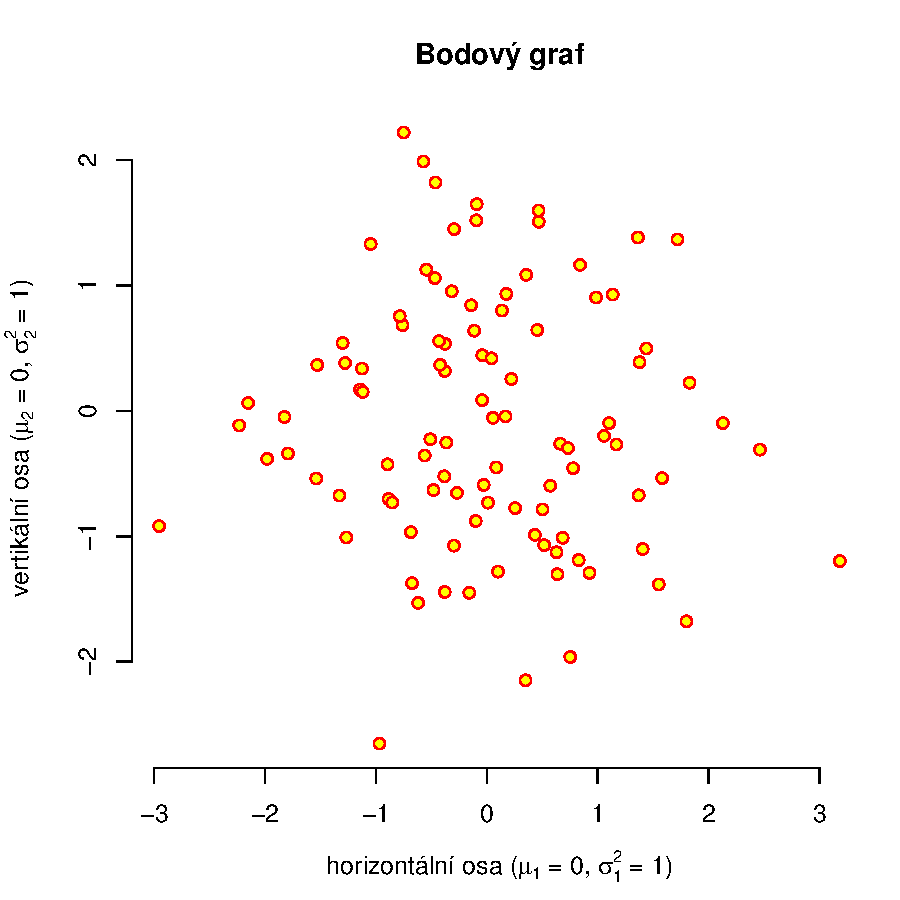
\includegraphics[width=140mm, height=140mm]{../img/ukazka-obr01}
% Příponu není potřeba explicitně uvádět, pdflatex automaticky hledá pdf.
% Rozměry také není nutné uvádět.
\caption{Náhodný výběr z~rozdělení $\mathcal{N}_2(\boldsymbol{0},\,I)$.}
\label{obr03:Nvyber}

\end{figure}

\begin{figure}[p]\centering
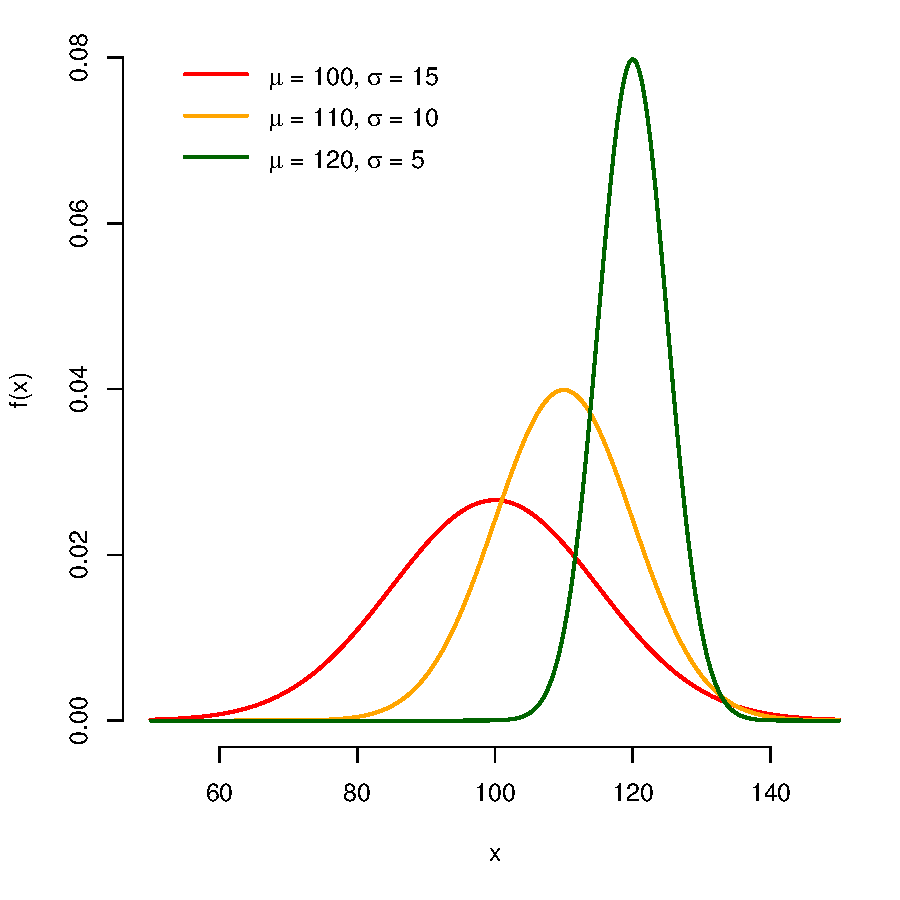
\includegraphics[width=140mm, height=140mm]{../img/ukazka-obr02}
\caption{Hustoty několika normálních rozdělení.}
\label{obr03:Nhust}
\end{figure}

\begin{figure}[p]\centering
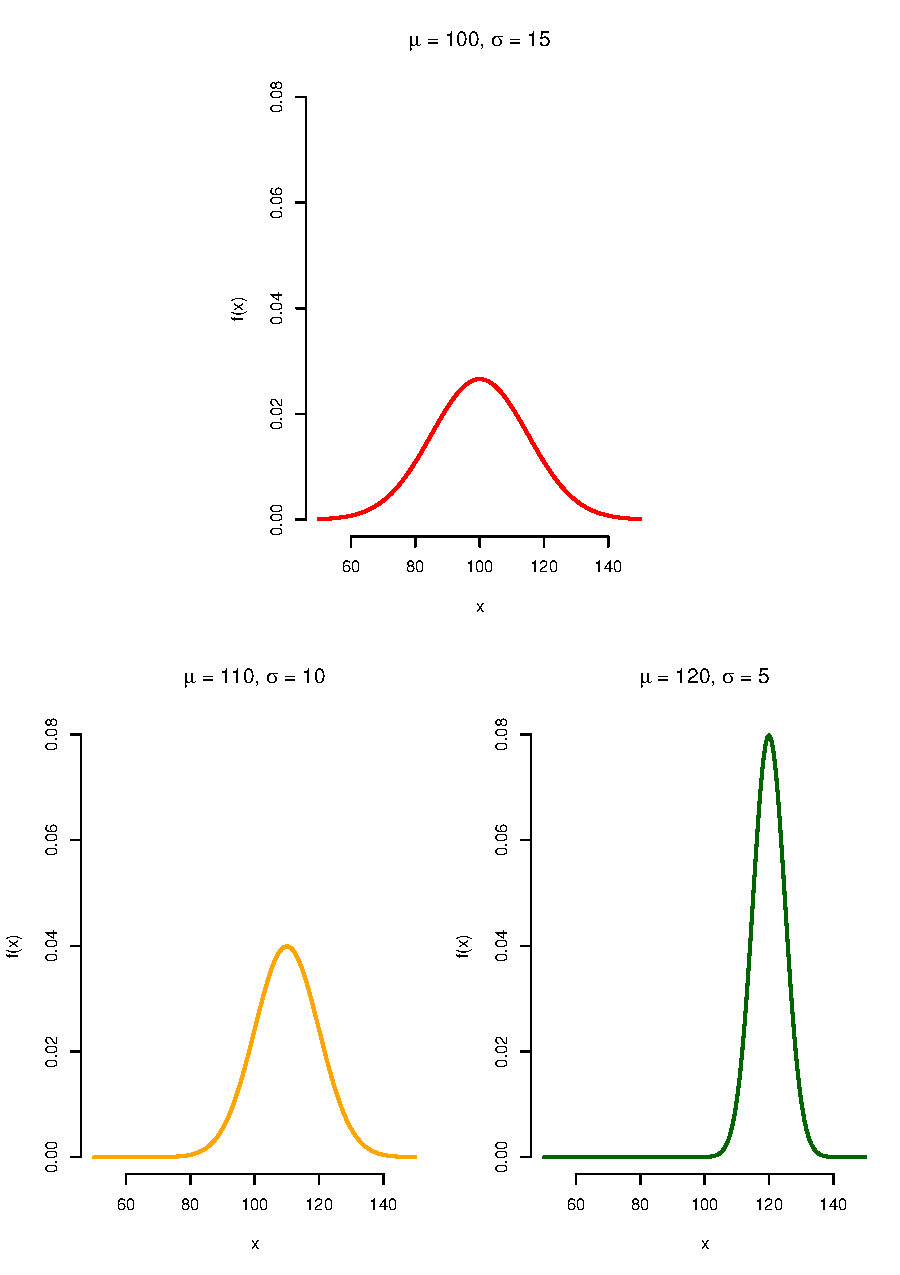
\includegraphics[width=140mm, height=198mm]{../img/ukazka-obr03}
\caption{Hustoty několika normálních rozdělení.}
\label{obr03:Nhust:podruhe}

\end{figure}
